\section*{Aufgabe 2 (25 Punkte)}
\vspace{0.4cm}
\subsection*{\nummer{a1}{4}}
Gegeben ist die Funktion
\begin{align*}
f \ : \ D_f \to \mathbb{R}, \ \ \
x \mapsto y = \sin(2x) 
\end{align*}
Bestimmen Sie das Taylorpolynom $P_3(x)$ dritter Ordnung von $f$ im Punkt $x_0 = \pi$.
\\
\\
\textbf{Lösung:}
\begin{mdframed}
\underline{\textbf{Vorgehensweise:}}
\begin{enumerate}
\item Überlege, was du für das dritte Taylorpolynom in $x_0=\pi$ berechnen musst.
\item Berechne dies und gebe das Taylorpolynom dritter Ordnung an. 
\end{enumerate}
\end{mdframed}
\underline{1. Überlege, was du für das dritte Taylorpolynom in $x_0=0$ berechnen musst. }\\
Die allgemeine Formel für das $n$-te Taylorpolynom ist durch
\begin{align*}
P_n(x) = \sum \limits_{k=0}^n \frac{f^{(k)}(x_0)}{k!} \cdot (x-x_0)^k
\end{align*}
gegeben. Also müssen wir
\begin{align*}
P_3(x) 
= f(x_0) + \frac{f^\prime(x_0)}{1!}\cdot (x-x_0) + \frac{f^{\prime \prime}(x_0)}{2!}\cdot (x-x_0)^2+
\frac{f^{\prime \prime \prime}(x_0)}{3!} \cdot (x-x_0)^3
\end{align*}
berechnen.
\\
\\
\underline{2. Berechne dies und gebe das Taylorpolynom dritter Ordnung an}\\
Durch 
\begin{align*}
f^\prime(x) = 2 \cos(2x), \
f^{\prime \prime}(x) = -4 \sin(2x), \
f^{\prime \prime \prime}(x) = -8 \cos(2x)
\end{align*}
erhalten wir die nötigen Ableitungen.
Damit erhalten wir 
\begin{align*}
f(\pi) = 0, \ f^\prime(\pi)= 2, \
f^{\prime \prime}(\pi) = 0, \
f^{\prime \prime \prime}(\pi) = -8
\end{align*}
als Werte.
Insgesamt ergibt sich
\begin{align*}
P_3(x) &= 2 \cdot (x - \pi) -\frac{8}{6} \cdot (x - \pi)^3\\
&= 2 \cdot (x - \pi) - \frac{4}{3} \cdot (x - \pi)^3
\end{align*}
als Taylorpolynom dritter Ordnung.

\newpage

\subsection*{\nummer{a2}{3}}
Gegeben ist die Funktion
\begin{align*}
f \ : \ D_f \to \mathbb{R}, \ \ \
x \mapsto y = \sin(2x) 
\end{align*}
$R_3(x)$ bezeichne das Restglied dritter Ordnung von $f$ in $x_0= \pi$.
Zeigen Sie, dass für $x \in [\pi -0.1, \pi+0.1]$ gilt:
\begin{align*}
|R_3(x)| \leq \frac{1}{10^4}.
\end{align*}
\textbf{Lösung:}
\begin{mdframed}
\underline{\textbf{Vorgehensweise:}}
\begin{enumerate}
\item Erinnere dich, was der Satz von Taylor über das Restglied des $n$-ten Taylorpolynoms aussagt. 
\item Berechne die vierte Ableitung von $f$ und suche eine passende Abschätzung dafür.
\item Finde eine geschickte Abschätzung für das Restglied. 
\end{enumerate}
\end{mdframed}

\underline{1. Erinnere dich, was der Satz von Taylor über das Restglied des $n$-ten Taylorpolynoms aussagt.}\\
Das Restglied des $n$-ten Taylorpolynoms ist durch
\begin{align*}
R_n(x) = \frac{f^{(n+1)}(\xi)}{(n+1)!}\cdot (x -x_0)^{n+1}
\end{align*}
für ein  $\xi$ zwischen $x_0$ und $x$ gegeben.\\
\\

\underline{2. Berechne die vierte Ableitung von $f$ und suche eine passende Abschätzung dafür}\\
Die vierte Ableitung von $f$ ist durch
\begin{align*}
f^{(4)}(x) =(-8 \cos(2x))^\prime = 16 \cdot \sin(2x)
\end{align*}
gegeben.\\
\\
%Hierfür können wir sogar
%\begin{align*}
%|f^{(4)}(x)| = |16 \sin(2x) | = 16 | \sin(2x)| \leq 16 \cdot 1
%\end{align*}
%abschätzen.

\underline{3. Finde eine geschickte Abschätzung für das Restglied}\\
Unser Restglied ist durch
\begin{align*}
R_3(x) = \frac{16  \sin(2\xi)}{4!} \cdot ( x - \pi)^4
= \frac{16  \sin(2\xi)}{24} \cdot ( x - \pi)^4
= \frac{2  \sin(2\xi)}{3} \cdot ( x - \pi)^4
\end{align*}
für ein $\xi$ zwischen $\pi$ und $x$ gegeben.
Der Betrag $| x - \pi |$ kann als Abstand von $x$ zu $\pi $ interpretiert werden.
Für $x \in [\pi - 0.1, \pi+0.1]$ erhalten wir
\begin{align*}
|x - \pi | < \frac{1}{10}
\end{align*}
als Hilfsabschätzung.
Für das Restglied gilt nun
\begin{align*}
|R_3(x)|= \left| \frac{2  \sin(2\xi)}{3} \cdot ( x - \pi)^4 \right| 
=\frac{2  | \sin(2 \xi) |}{3} \cdot |x-\pi|^4
= \frac{2}{3} \underbrace{|\sin(2 \xi)|}_{\leq 1} \cdot \underbrace{|x - \pi|}^4_{\leq \left(\frac{1}{10}\right)^4}
\leq \frac{2}{3} \cdot \frac{1}{10^4}
\leq \frac{1}{10^4}
\end{align*}
für $x \in [\pi - 0.1, \pi +0.1]$. 


\newpage

\subsection*{\nummer{b}{4}}
Gegeben ist die Funktion
\begin{align*}
f(x,y) = 
\ln(4 \ x^2 + y^2- 16) + \sqrt[3]{25 - x^2 - y^2}. 
\end{align*}
Ermitteln Sie den Definitionsbereich $D_f$ von $f$
und stellen Sie diesen graphisch dar.
\\
\\
\textbf{Lösung:}
\begin{mdframed}
\underline{\textbf{Vorgehensweise:}}
\begin{enumerate}
\item Überlege dir, welche Bedingungen für den Definitionsbereich erfüllt sein müssen.
\item Gebe den Definitionsbereich an. 
\item Skizziere den Definitionsbereich. 
\end{enumerate}
\end{mdframed}

\underline{1. Überlege dir, welche Bedingungen für den Definitionsbereich erfüllt sein müssen}\\
Die erste Bedingung ist durch
\begin{align*}
4 \ x^2 + y^2 -16 > 0
\Leftrightarrow
4 \ x^2 + y^2 > 16
\Leftrightarrow
\frac{x^2}{4} + \frac{y^2}{16} > 1
\Leftrightarrow
\frac{x^2}{2^2} + \frac{y^2}{4^2} > 1 
\end{align*}
gegeben.
Eine Gleichung der Form 
\begin{align*}
\frac{x^2}{a^2} + \frac{y^2}{y^2} = 1
\end{align*}
beschreibt eine Ellipse um den Ursprung durch die Punkte $(\pm a , 0)$ und $(0, \pm b)$.
Für die zweite Bedingung erhalten wir durch
\begin{align*}
25 -x^2 -y^2 \geq 0
\Leftrightarrow
x^2 + y^2 \leq  25 = 5^2
\end{align*}
eine Kreisgleichung.
Eine Gleichung der Form 
\begin{align*}
x^2 + y^2 =r^2
\end{align*}
beschreibt einen Kreis um den Ursprung mit Radius $r$.
Beide Bedingungen zusammen ergeben eine Kreisscheibe mit ausgeschnittener Ellipse.\\
\\
\underline{2. Gebe den Definitionsbereich an}\\
Wir können nun den Definitionsbereich von $f$ durch
\begin{align*}
D_f
=
\left\lbrace (x,y) \ | \ 
\frac{x^2}{2^2} + \frac{y^2}{4^2} > 1
\ \text{und} \
x^2 + y^2 \leq 5^2 \right\rbrace
\end{align*}
angeben.
\\
\\
\newpage
\underline{3. Skizziere den Definitionsbereich}\\

\pgfplotsset{compat=1.3,compat/path replacement=1.5.1}
\begin{figure}[h]
\centering
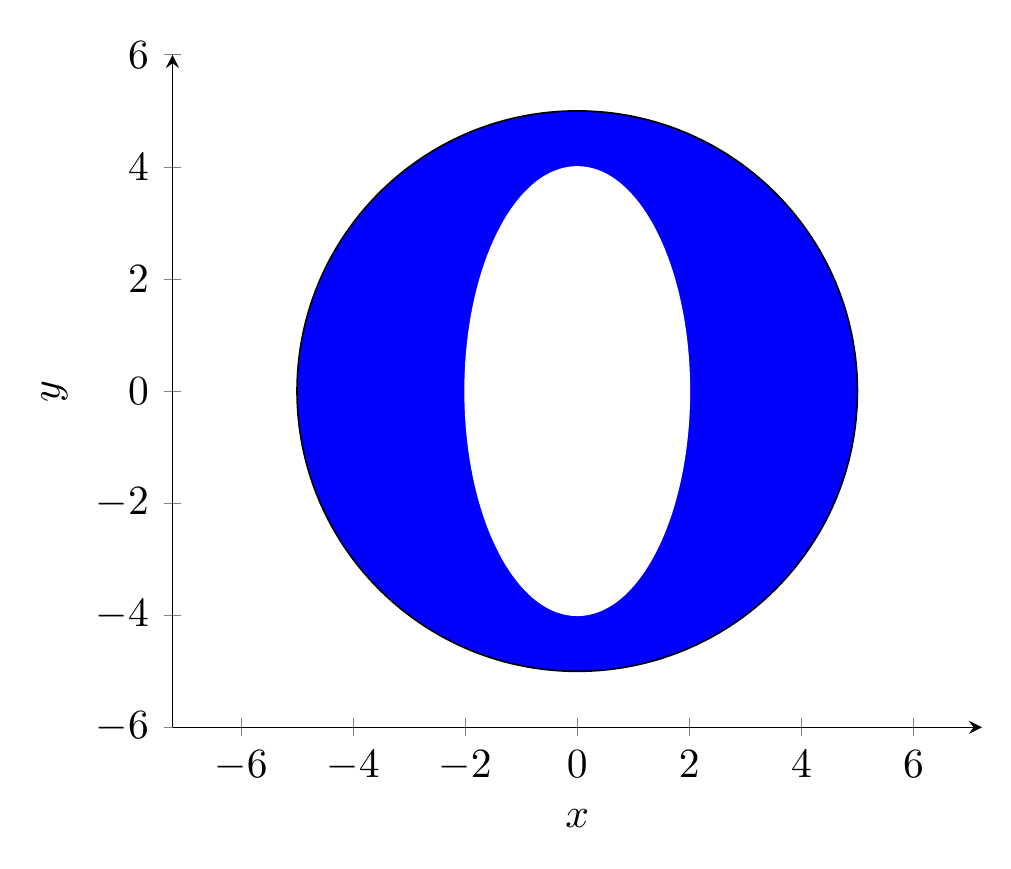
\begin{tikzpicture}[scale=1.5]

\begin{axis}[
        axis lines = left,
        xmin=-6, xmax=6, ymin=-6, ymax=6,
        axis equal,
        xlabel = $x$,
        ylabel = {$y$}]
        \draw[fill=blue] (axis cs: 0, 0) circle [radius=5];
         
        \draw[white, fill = white] (axis cs:0,0) ellipse [ x radius=2, y radius=4];
    \end{axis}
\end{tikzpicture}
\end{figure}

\newpage

\subsection*{\nummer{c}{4}}
Gegeben ist die Funktion
\begin{align*}
f(x,y) = \cos(x) \ \sin(y) + a \ (x+3)^2.
\end{align*}
Für welches $a \in \mathbb{R}$ nimmt die Tangentensteigung
an die Niveaulinie im Punkt $(x_0,y_0) = ( 0, \pi) $
den Wert $3$ an?\\
\\ 
\textbf{Lösung:}
\begin{mdframed}
\underline{\textbf{Vorgehensweise:}}
\begin{enumerate}
\item Überlege dir, wie du die Tangentensteigung an die Niveaulinie angeben kannst.

\item Überlege dir, welcher Satz angewendet werden muss.

\item Berechne $a$.

   
\end{enumerate}
\end{mdframed}

\underline{1. Überlege dir, wie du die Tangentensteigung an die Niveaulinie angeben kannst}\\
Die Tangentensteigung an die Niveaulinie im Punkt $(x_0,y_0)$
ist durch
\begin{align*}
\frac{\td{y}}{\td{x}} \bigg|_{(x_0,y_0)}
\end{align*}
gegeben.
Wir müssen also die Gleichung
\begin{align*}
\frac{\td{y}}{\td{x}} \bigg|_{(0,\pi)} =  3
\end{align*}
lösen.\\
\\

\underline{2. Überlege dir, welcher Satz angewendet werden muss}\\
Über den Satz der impliziten Funktionen erhalten wir
\begin{align*}
\frac{\td{y}}{\td{x}} \bigg|_{(0,\pi)} 
=
-\frac{f_x(0,\pi)}{f_y(0,\pi)} =3
\end{align*}
als Ansatz.
\\
\\

\underline{3. Berechne $a$}\\
Zunächst berechnen wir durch
\begin{align*}
f_x(x,y) &= -\sin(x) \cdot \sin(y) + 2a \cdot (x+3) \\
f_y(x,y) &= \cos(x) \cdot \cos(y)
\end{align*}
die partiellen Ableitungen.
Eingesetzt in unseren Ansatz ergibt dies
\begin{align*}
-\frac{f_x(0,\pi)}{f_y(0,\pi)}
= 
\frac{\sin(0)\cdot \sin(\pi)-2a \cdot(0+3)}{\cos(0) \cdot \cos(\pi)}
= 
\frac{-0 \cdot 0 - 2a\cdot 3}{1 \cdot (-1)}
=
\frac{-6a}{-1}
= \frac{6a}{1} = 6a.
\end{align*}
das gesuchte $a$.
Jetzt setzen wir diese Termumformung gleich $3$ und erhalten mit
\begin{align*}
6a = 3 \Leftrightarrow a = \frac{3}{6} = \frac{1}{2}
\end{align*}
das gesuchte $a$.
\newpage

\subsection*{\nummer{d1}{3}}
Gegeben ist die Produktionsfunktion
\begin{align*}
P(K,A)= 
8  \left( \frac{\lambda}{K} +\frac{1}{2A} \right)^{-0.5}
\quad ( \lambda >0 ).
\end{align*}
Berechnen Sie die Grenzerträge $P_K$ und $P_A$
sowie die partiellen Elastizitäten 
$\varepsilon_{P,K}$ und $\varepsilon_{P,A}$.
\\
\\ 
\textbf{Lösung:}
\begin{mdframed}
\underline{\textbf{Vorgehensweise:}}
\begin{enumerate}
\item Berechne die Grenzerträge $P_K$ und $P_A$.
\item Berechne die partiellen Elastizitäten.
\end{enumerate}
\end{mdframed}

\underline{1. Berechne die Grenzerträge $P_K$ und $P_A$}\\
Die Grenzerträge entsprechen jeweils den partiellen Ableitungen.
Damit erhalten wir durch die Kettenregel
\begin{align*}
P_K(K,A)
&= 8 \cdot (-0.5) \ \left( \frac{\lambda}{K} +\frac{1}{2A} \right)^{-1.5} \cdot \frac{-\lambda}{K^2}
= 4 \lambda \  \left( \frac{\lambda}{K} +\frac{1}{2A} \right)^{-1.5} \cdot \frac{1}{K^2}
= \frac{4 \ \lambda}{K^2} \  \left( \frac{\lambda}{K} +\frac{1}{2A} \right)^{-1.5}\\ 
P_A(K,A) &= 8 \cdot (-0.5) \ \left( \frac{\lambda}{K} +\frac{1}{2A} \right)^{-1.5}
\cdot \frac{-1}{2 \ A^2}
= 4 \ \left( \frac{\lambda}{K} +\frac{1}{2A} \right)^{-1.5}
\cdot \frac{1}{2 \ A^2}
= \frac{2}{ A^2} \ \left( \frac{\lambda}{K} +\frac{1}{2A} \right)^{-1.5}
\end{align*}
die gesuchten Grenzerträge.\\
\\

\underline{2. Berechne die partiellen Elastizitäten}\\
Für die partiellen Elastizitäen gilt
\begin{align*}
\varepsilon_{P,K}(K,A) = \frac{P_K(K,A)}{P(K,A)} K
\ \text{und} \
\varepsilon_{P,A}(K,A) =  \frac{P_A(K,A)}{P(K,A)} A,
\end{align*}
wodurch wir mit Einsetzen 
\begin{align*}
\varepsilon_{P,K}(K,A) 
&=  \frac{\frac{4 \ \lambda}{K^2}  \  \left( \frac{\lambda}{K} +\frac{1}{2A} \right)^{-1.5} }{8 \ \left( \frac{\lambda}{K} +\frac{1}{2A} \right)^{-0.5}} K
= \frac{4 \ K \ \lambda}{8 \ K^2} \cdot \left( \frac{\lambda}{K} +\frac{1}{2A} \right)^{-1}
= \frac{ \lambda}{2 \ K} \cdot \left( \frac{\lambda}{K} +\frac{1}{2A} \right)^{-1} \\
\varepsilon_{P,A}(K,A)
&=  \frac{\frac{2}{ A^2}  \ \left( \frac{\lambda}{K} +\frac{1}{2A} \right)^{-1.5}}{8 \ \left( \frac{\lambda}{K} +\frac{1}{2A} \right)^{-0.5}} A
= \frac{1}{4 \ A} \ \left( \frac{\lambda}{K} +\frac{1}{2A} \right)^{-1} 
\end{align*}
die richtigen Resultate erhalten.
\newpage

\subsection*{\nummer{d2}{3}}
Gegeben ist die Produktionsfunktion
\begin{align*}
P(K,A)= 
8 \ \left( \frac{\lambda}{K} +\frac{1}{2A} \right)^{-0.5}
\end{align*}
mit $\lambda = 2$.\\
Berechnen Sie das totale Differential $\td{P}$ von $P$
in $(K_0,A_0)= \left( 1, \frac{1}{4} \right)$.\\
Berechnen Sie mit Hilfe des totalen Differentials einen Näherungswert für $P(0.98,0.29)$.
\\
\\ 
\textbf{Lösung:}
\begin{mdframed}
\underline{\textbf{Vorgehensweise:}}
\begin{enumerate}
\item Berechne das totale Differential.
\item Approximiere mit Hilfe des totalen Differentials $P(0.98,0.29)$.
\end{enumerate}
\end{mdframed}

\underline{1. Berechne das totale Differential}\\
Mit dem Zusammenhang
\begin{align*}
P(0.98,0.29) \approx  P(1,0.25) + \td{P}
\end{align*}
erhalten wir 
\begin{align*}
\td{P} = P_K(1,0.25) \ \td{K} + P_A(1,0.25)  \ \td{A} 
\end{align*}
und
\begin{align*}
\td{K} = 0.98 - 1 = -0.02
\ \text{und} \
\td{A} = 0.29 - 0.25 = 0.04. 
\end{align*}
Mit 
\begin{align*}
P_K(1,0.25) &= 
\frac{8}{1} \left( 2 + \frac{1}{0.5} \right)^{-1.5}
= \frac{8}{\sqrt{(2 +2)^3}}
= \frac{8}{\sqrt{4^2} \cdot \sqrt{4}}
= \frac{8}{8}
= 1
\\
P_A(1,0.25)
&= \frac{2}{(0.25)^2} \cdot \frac{1}{8}
= \frac{2}{\frac{1}{16}} \cdot \frac{1}{8} 
= 32 \cdot \frac{1}{8} = 4
\end{align*}
erhalten wir durch Einsetzen in das Differential
\begin{align*}
\td{P} = - 0.02 + 4 \cdot 0.04
= -0.02 + 0.16 = 0.14
\end{align*}
den Wert für $\td{P}$.\\
\\

\underline{2. Approximiere mit Hilfe des totalen Differentials $P(0.98,0.29)$ }\\
Durch 
\begin{align*}
P(1,0.25) =
8 \ \left( \frac{2}{1} +\frac{1}{0.5} \right)^{-0.5}
=
\frac{8}{\sqrt{2 + 2}}
=
\frac{8}{\sqrt{4}}
=
\frac{8}{2}
=
4
\end{align*}
erhalten wir
\begin{align*}
P(0.98,0.29) \approx 4 + 0.14 = 4.14
\end{align*}
eine geeignete Approximation.


\newpage

\subsection*{\nummer{d3}{4}}
Gegeben ist die Produktionsfunktion
\begin{align*}
P(K,A)= 
8 \ \left( \frac{\lambda}{K} +\frac{1}{2A} \right)^{-0.5}.
\end{align*}
Für welche Werte von $\lambda \in \mathbb{R}_+$ ist die technische Substitutionsrate im Punkt $(K_0,A_0) = \left( 1, \frac{1}{4} \right)$ gleich $-1$.
\\
\\ 
\textbf{Lösung:}
\begin{mdframed}
\underline{\textbf{Vorgehensweise:}}
\begin{enumerate}
\item Bestimme die technische Substitutionsrate mit Hilfe des Satzes über implizite Funktionen.
\end{enumerate}
\end{mdframed}

\underline{1. Bestimme die technische Substitutionsrate mit Hilfe des Satzes über implizite Funktionen}\\
Die technische Substitutionsrate ist durch
\begin{align*}
\frac{\td{A}}{\td{K}}
\end{align*}
gegeben. Wir erhalten
\begin{align*}
\frac{\td{A}}{\td{K}} \bigg|_{(K_0,A_0)} =
-\frac{P_K(K_0,A_0)}{P_A(K_0,A_0)} 
\end{align*}
durch den Satz über implizite Funktionen. 
Eingesetzt erhalten wir 
\begin{align*}
\frac{\td{A}}{\td{K}} \bigg|_{(K,A)}
= 
-\frac{\frac{4 \ \lambda}{K^2} \  \left( \frac{\lambda}{K} +\frac{1}{2A} \right)^{-1.5}}{\frac{2}{ A^2} \ \left( \frac{\lambda}{K} +\frac{1}{2A} \right)^{-1.5}}
= -\frac{\frac{4 \ \lambda}{K^2}}{\frac{2}{A^2}}
= -\frac{4 \ \lambda \ A^2}{2 \ K^2}
= -\frac{2 \ \lambda \ A^2}{K^2},
\end{align*}
wodurch für $(1,0.25)$
\begin{align*}
\frac{\td{A}}{\td{K}} \bigg|_{(1,0.25)}
= -\frac{2 \ \lambda \ (0.25)^2}{1}
= -2 \lambda\frac{1}{16}
= \frac{-\lambda}{8}
\end{align*}
folgt. Insgesamt erhalten wir durch 
\begin{align*}
-\frac{\lambda}{8} = -1
\Leftrightarrow
\lambda = 8
\end{align*}
das gesuchte $\lambda$.

\newpage